\documentclass[a4paper,fleqn,twoside]{article}

\usepackage[pdftex]{graphicx,xcolor}
\usepackage[font=small,skip=3pt]{caption}

\usepackage[T1]{fontenc}
\usepackage{lmodern}
\usepackage{amsfonts}

%
\usepackage{tocloft}

% Turn off paragraph indentation 
\usepackage{parskip}

% Title page stuff
\usepackage{eso-pic}
\usepackage[absolute]{textpos}

% Hide page number on empty pages
\usepackage{emptypage}

% Verbatim with support for line breaks
\usepackage{fancyvrb}
\usepackage{fvextra}

% Split long sequences
\usepackage{seqsplit}

% Support for sub-figures and tables
\usepackage{subcaption}

% Support for multirow tables
\usepackage{multirow}

% Support aplh. lists
\usepackage{enumitem}

%% Support for colored text box
%\usepackage{mdframed}

% Support for highlighted code
\usepackage{listings}

% Support keys
\usepackage{menukeys}

% Set used page surface
%\usepackage[showframe]{geometry}
%\usepackage[a4paper,left=3cm,right=2cm,top=2.5cm,bottom=2.5cm]{geometry}
\usepackage[a4paper,inner=4.5cm,outer=3.5cm,top=4.0cm,bottom=4.5cm]{geometry}

% imakeidx: Allows to create separate indexes for input parameters and other items
\usepackage{imakeidx}
\makeindex[name=prmindex, title={Index of input parameters\label{sec:index inputs}}]
\makeindex[name=prmindexfull, title={Index of input parameters\label{sec:index inputs full}}]

% hyperref: set the base for relative links to the top-level \dftfe directory so that we can link to files in the \dftfe tree without having to specify the location relative to the directory where the pdf actually resides
\usepackage[colorlinks,linkcolor=blue,urlcolor=blue,citecolor=blue,baseurl=../]{hyperref}
\newcommand{\whitehref}[3][white]{\href{#2}{\color{#1}{#3}}}%

% Set \today command to display: month, year
\renewcommand{\today}{\ifcase \month \or January\or February\or March\or April\or May\or June\or July\or August\or September\or October\or November\or December\fi, \number \year} 


% Rounded 'menu' keys
\renewmenumacro{\menu}[>]{roundedmenus}

% Square 'tabmenu' keys
\makeatletter
\tw@declare@style*{mystyle}{% Fist item
	\tikz[baseline={($(tw@node.base)+(0,-0.2ex)$)}]{%
		\node(tw@node)[tw@angularmenus@base,font=\relsize{-1}\normalfont\bfseries,signal to=east,fill=gray!30]%
		{\strut\CurrentMenuElement};}%
}[\hspace{-0.2em}\hspace{0em plus 0.1em minus 0.05em}]%
{% Intermediate items
	\tikz[baseline={($(tw@node.base)+(0,-0.2ex)$)}]{%
		\node(tw@node)[tw@angularmenus@base,font=\relsize{-1}\normalfont,signal from=west,signal to=east]%
		{\strut\CurrentMenuElement};}%
}{% Last item
	\tikz[baseline={($(tw@node.base)+(0,-0.2ex)$)}]{%
		\node(tw@node)[tw@angularmenus@base,font=\relsize{-1}\normalfont,signal from=west]%
		{\strut\CurrentMenuElement};}%
}{% Other items
	\tikz[baseline={($(tw@node.base)+(0,-0.2ex)$)}]{%
		\node(tw@node)[tw@angularmenus@base,font=\relsize{-1}\normalfont\bfseries,fill=gray!30]{\strut\CurrentMenuElement};}%
}{gray}
\makeatother
\newmenumacro{\tabmenu}[>]{mystyle}


% Macro defining highlighting rules for YAML [listings]
\makeatletter
%
\newcommand\language@yaml{yaml}
% Define highlighting colors
\definecolor{YAMLbackground}{rgb}{1,1,1} % white
\definecolor{YAMLdefault}{RGB}{0,0,0} % black
\definecolor{YAMLcomment}{RGB}{0,128,0} % green
\definecolor{YAMLidentifier}{RGB}{0,0,128} % blue
\definecolor{YAMLnumber}{RGB}{255,128,64} % orange
\definecolor{YAMLtext}{RGB}{128,128,128} % grey
% Expand macro
\expandafter\expandafter\expandafter\lstdefinelanguage
\expandafter{\language@yaml}
{	identifierstyle=\ttfamily,
	commentstyle=\color{YAMLcomment},
	stringstyle=\color{YAMLtext},
	basicstyle=\fontsize{8}{8}\selectfont\ttfamily\color{YAMLidentifier}, % Assuming a key comes first
	numbers=none, % Position of the line numbers
	%stepnumber=1,
	%numbersep=10pt,
	tabsize=2, % Default tabsize
	breaklines=true, % Automatic line break
	frame=single,
	backgroundcolor=\color{YAMLbackground}, % Background color
	sensitive=false,
	comment=[l]{\#},
	moredelim=**[il][\color{YAMLidentifier}{:}\color{YAMLdefault}]{:}, % Switch to value style at :
	morestring=[b]',
	morestring=[b]",
}
% Switch to key style at EOL
\lst@AddToHook{EveryLine}{\ifx\lst@language\language@yaml\color{YAMLdefault}\fi}
\makeatother

% User defined commands
\newcommand{\asli}{\textsc{ASLI}}
\newcommand{\qasli}{\textsc{QASLI}}
\newcommand{\mycirc}[1][black]{\small\textcolor{#1}{\ensuremath\bullet}} % Colored bullet point

% Document user defined colors
\definecolor{titlepagecolor}{rgb}{0.95,0.95,0.96}
\definecolor{marineBlue}{RGB}{66,111,128}
\definecolor{myColorA}{HTML}{7d1700}%125/23/0
\definecolor{myColorB}{HTML}{a86000}%168/96/0
\definecolor{myColorC}{HTML}{cebe36}%206/190/54
\definecolor{myColorD}{HTML}{3dc8d6}%61/200/214
\definecolor{myColorE}{HTML}{0070ba}%0/112/186
\definecolor{myColorF}{HTML}{002f98}%0/47/152

% 
\begin{document}
	\newgeometry{left=0cm,right=0cm,top=0.3cm,bottom=0.3cm}
\begin{titlepage}
	%\pagecolor{titlepagecolor}
	
	\AddToShipoutPictureBG*{\AtPageLowerLeft{%
	\color{marineBlue}\rule{.3\paperwidth}{\paperheight}}}
	
	\vspace*{16.0em}
	
	% Title block
	\begin{textblock*}{20em}(18.0em,16.0em)
		\begin{minipage}{40em}
			\begin{center}
				
\includegraphics[height=10.5em]{figures/ASLI.png}\\[10pt]
				{\Large A Simple Lattice Infiller}
				\vspace{3.0em}
				
				\Huge User Manual
				\vspace{0.2em}
				
				\Large (\today)
			\end{center}
		\end{minipage}
	\end{textblock*}

	\vfill
	
	% Footer
	\begin{center}
		\begin{tabular*}{0.97\textwidth}{@{}l@{\extracolsep{\fill}}r@{}}
			& \multirow[b]{3}{*}{
				
\includegraphics[height=1.3cm]{figures/KUL.png}
			} \\
			 \whitehref{http://www.biomech.ulg.ac.be/ASLI/}{\large \asli{} website} & \\
			 \whitehref{https://github.com/tpms-lattice}{\large \asli{} github repository} &
		\end{tabular*}\\
	
		{\noindent \color{black}\rule{\textwidth}{1.7pt}}\\[3pt] % Line
		
		\begin{tabular*}{0.97\textwidth}{@{}l@{\extracolsep{\fill}}r@{}}
			\large ASLI Version 0.1 & Copyright (c) 2019-\the\year, KU Leuven
		\end{tabular*}
	\end{center}
	
\end{titlepage}
\restoregeometry
	\clearpage%\cleardoublepage

	\pagenumbering{roman} % Start roman numbering
	
	% Contents
	\tableofcontents
	\clearpage%\cleardoublepage
	
	\pagenumbering{arabic} % Switch to arabic numbers
	
	% Introduction
	\section{Introduction} \label{sec:intro}
\asli{} (A Simple Lattice Infiller) is a cross-platform command line open-source tool written in C++ that gives users the ability to provide functionally graded lattice infills to any 3D geometry. The lattice infill is constructed out of unit cells, described by implicit functions, whose type, size and feature can be varied locally to obtain the desired local properties. \asli{} also has an optional Graphical User Interface (GUI) available, called \qasli{}.

Details on the technical aspects of \asli{} can be found in ``\href{https://doi.org/10.1080/17452759.2022.2048956}{A flexible and easy-to-use open-source tool for designing functionally graded 3D porous structures}''.

\subsection{Authors} \label{sec:authors}
\asli{} and \qasli{} are developed by the \href{http://www.biomech.ulg.ac.be}{Biomechanics Research Unit} (University of Li\`{e}ge and KU Leuven). %Both are currently maintained by their principal developers.

\paragraph*{Principal developers}
\begin{itemize}
	\item F. Perez-Boerema [Developer of \asli{}] (KU Leuven, Belgium)
	\item M. Barzegari [Developer of \qasli{}] (KU Leuven, Belgium)
\end{itemize}

\paragraph*{Principal investigator}
\begin{itemize}
	\item L. Geris (University of Li\`{e}ge and KU Leuven, Belgium)
\end{itemize}

\subsection{Licensing} \label{sec:licensing}
\asli{} is licensed under the terms of the GNU Affero General Public License.

\subsection{Citing \asli{}}
If you use \asli{} for your research we kindly ask you to cite:
\begin{itemize}
	\item F. Perez-Boerema, M. Barzegari and L. Geris. (2022). A flexible and easy-to-use open-source tool for designing functionally graded 3D porous structures, \textit{Virtual and Physical Prototyping}, 17:3, 682-699, DOI: \href{https://doi.org/10.1080/17452759.2022.2048956}{\seqsplit{10.1080/17452759.2022.2048956}}.
	
\end{itemize}

\subsection{Acknowledgments}
The authors gratefully acknowledge funding from the European Regional Development Fund – Interreg VA Flanders - The Netherlands (PRosPERoS, CCI 2014\-TC\-16\-RFCB\-046), the European Union’s Horizon 2020 research and innovation programme via the European Research Council (ERC CoG INSITE 772418), the Fund for Scientific Research Flanders (G085018N), the Fédération Wallonie-Bruxelles through the BioWin project BIOPTOS (7560) and the KU Leuven Special Research Fund (C24/17/07).
	
	% Installation
	\section{Getting started} \label{sec:installation}
The easiest way to get started with \asli{} is to use its pre-build binaries. To this end, all you need to do is download the tarballs for your preferred platform (Linux or Windows) from the \href{https://github.com/tpms-lattice/ASLI/releases}{release page} of \href{https://github.com/tpms-lattice/ASLI}{\asli{} repository}, unpack them and if using Linux install oneTBB if not available on your system (only required by the parallel version of \asli{}). The tarball contains \asli{}, including its GUI. For more advanced advanced users, it may be more interesting to build \asli{} from scratch. Not only is this likely to increase performance since the program will get optimized for the platform in which it is going to be run, but it will also enable users to customize \asli{} in any way they need. The prerequisites to be able to build \asli{} are detailed in Section~\ref{sec:prerequisites}, while the procedure to build \asli{} is detailed in Section~\ref{sec:buildLin} and \ref{sec:buildWin}, for Linux and Windows respectively. 

\subsection{Prerequisites} \label{sec:prerequisites}
\asli{} makes use of \href{http://www.cmake.org}{CMake} and \href{https://www.gnu.org/software/make/}{GNU Make} to automate the building process. It also has a series of dependencies, which are listed below.
\begin{itemize}
	\item \href{https://github.com/ISCDtoolbox/AdaptTools}{AdaptTools}
	\item \href{https://www.alglib.net}{ALGLIB}
	\item \href{https://www.cgal.org}{CGAL}
	\begin{itemize}
		\item \href{https://gmplib.org}{GMP}
		\item \href{https://www.mpfr.org}{MPFR}
		\item \href{https://www.boost.org}{Boost}
		\item \href{http://intel.com/oneTBB}{oneTBB} (optional, required for parallelization)
	\end{itemize}
	\item \href{http://eigen.tuxfamily.org}{Eigen}
	\item \href{https://www.mmgtools.org}{MMG}
	\item \href{http://tetgen.org}{TETGEN}
	\item \href{https://github.com/jbeder/yaml-cpp}{Yaml-cpp}
	\item \href{https://github.com/tpms-lattice/QASLI}{\qasli{}} (optional, the GUI of \asli{})
	\begin{itemize}
		\item \href{https://www.qt.io}{QT} (optional, required if compiling the GUI)
	\end{itemize}
\end{itemize}

Most dependencies are included with \asli{} so that the user does not need to worry about them. Not included with \asli{} are GMP, MPFR, Boost and TBB (optional). QT, required to compile the GUI of \asli{} is not included either. To be able to compile \asli{}, depending on the compilation settings, users will need some or all of these libraries available on their system.

\subsection{Building \asli{} in Linux}\label{sec:buildLin}

If you are missing some required or optional dependencies they can be installed on Debian and Ubuntu with a couple of commands.

\begin{itemize}
	\item Install build tools:
		\begin{verbatim}
			$ sudo apt-get install git cmake
		\end{verbatim}

	\item Install compilers:
		\begin{verbatim}
			$ sudo apt-get install build-essential
		\end{verbatim}

	\item Install libraries (GMP, MPFR, Boost):
	\begin{verbatim}
		$ sudo apt-get install libgmp-dev libmpfr-dev libboost-all-dev
	\end{verbatim}

	\item Install libraries (oneTBB):
	\begin{verbatim}
		$ sudo apt-get install libtbb-dev
	\end{verbatim}

	\item Install libraries (QT):
	\begin{verbatim}
		$ sudo apt-get install qt3d5-dev
	\end{verbatim}
\end{itemize}

Once the build tools, compilers and required dependencies are available on the system the main steps to build \asli{} in Linux are the following.
\begin{enumerate}
	\item Retrieve ASLI from the repository:
		\begin{verbatim}
			$ git clone https://github.com/tpms-lattice/ASLI.git
		\end{verbatim}
	\item Compile:
		\begin{verbatim}
			$ cd ASLI
			$ mkdir build
			$ cd build
			$ cmake -DCMAKE_BUILD_TYPE=Release -DMARCH_NATIVE=ON ..
			$ make
		\end{verbatim}
\end{enumerate}

To clean up, simply delete the \texttt{build} and \texttt{bin} directories found in the source directory.

\subsection{Building \asli{} in Windows}\label{sec:buildWin}
Windows compilation is supported with \href{https://www.msys2.org/}{MSYS2}. Once you have \href{https://www.msys2.org/#installation}{installed MSYS2 in windows} the required and optional dependencies can be installed through the MSYS2 MinGW 64-bit terminal with a couple of commands.

\begin{itemize}
	\item Install build tools:  
	\begin{verbatim}
		$ pacman -S git mingw-w64-x86_64-cmake
	\end{verbatim}

	\item Install compilers, and libraries (GMP, MPFR, Boost):  
	\begin{verbatim}
		$ pacman -S --needed base-devel mingw-w64-x86_64-toolchain
		$ pacman -S msys2-runtime-devel
	\end{verbatim}

	\item Install libraries (oneTBB):
	\begin{verbatim}
		$ pacman -S mingw-w64-x86_64-intel-tbb
	\end{verbatim}
	and add the location of \texttt{tbb.dll} and \texttt{tbbmalloc.tbb} to the windows environment variables.

	\item Install libraries (QT):
	\begin{verbatim}
		$ pacman -S mingw-w64-x86_64-qt5
	\end{verbatim}
\end{itemize}

Once the build tools, compilers and required dependencies have been installed the main steps to build \asli{} for Windows in MSYS2 are the following.
\begin{enumerate}
	\item Retrieve ASLI from the repository:
		\begin{verbatim}
			$ git clone https://github.com/tpms-lattice/ASLI.git
		\end{verbatim}
	\item Compile:
		\begin{Verbatim}[breaklines=true, tabsize=0]
			$ cd ASLI
			$ mkdir build
			$ cd build
			$ cmake -G "MSYS Makefiles" -DCMAKE_BUILD_TYPE=Release -DMARCH_NATIVE=ON ..
			$ make
		\end{Verbatim}
\end{enumerate}

To clean up, simply delete the \texttt{build} and \texttt{bin} directories found in the source directory.

\subsection{Parallel mode}
To compile ASLI in parallel mode include the tag \verb|-DCGAL_|\hspace{0pt}\verb|ACTIVATE_|\hspace{0pt}\verb|CONCURRENT_|\hspace{0pt}\verb|MESH_3=ON| when calling cmake. Note that parallel mode is currently limited to the CGAL workflow.

\subsection{Graphical user interface}
To compile ASLI together with its GUI include the tag \verb|-DASLI_GUI=ON| when calling cmake.
	
	% Running ASLI
	\section{Using \asli} \label{sec:run}
After compiling \asli{} you will find an executable file named \texttt{ASLI} in the bin folder. If you specified you would like the GUI to be compiled along with \asli{} you will find a second executable in the bin folder named \texttt{QASLI}.

%or downloading its pre-build binaries

In order to call \asli{} from the command line you only need to type the following command in the Linux terminal:
\begin{verbatim}
	./ASLI config.yml
\end{verbatim}
or if using windows:
\begin{verbatim}
	ASLI.exe config.yml
\end{verbatim}
where \texttt{config.yml} points to the configuration file.

If using the GUI of \asli{} users will only need to open \qasli{}, through which all user input parameters can be specified prior to executing \asli{}.

\subsection{Configuration file} \label{sec:configuration}
\asli{} makes use of a YAML configuration file that can be edited in any text editor. Through this file users can specify the user input parameters. The structure of the configuration file is shown in Fig. \ref{fig:config} while a detailed description of each input parameter can be found in Appendix \ref{sec:parameters}.

\begin{figure}[htb]
\centering
\begin{minipage}{.9\linewidth}
%\lstinputlisting[frame=single,firstline=21,lastline=71,language=yaml]{../../config.yml}
\begin{lstlisting}[language=yaml]
# ----  CONFIGURATION FILE  ---- #

# Input & output files
files:
  stl: inputs/cube.stl
  tap: inputs/cube.tap
  sap: inputs/cube.sap
  fap: inputs/cube.fap
output: outputs/

# Lattice settings
lt_type: gyroid
lt_type_filterRadius: 1.0
lt_type_correctionFactor: 0.25

lt_size: 0.5

lt_feature: isovalue
lt_feature_val: 0.5
lt_feature_mode: relative

# Mesh settings
me_mesher: CGAL
me_side: scaffold
me_volumeMesh: FALSE
me_nThreads: 1

# Mesh settings (CGAL)
me_facetAngle: 0
me_facetSize: 0
me_facetDistance: 0.015
me_cellRadiusEdgeRatio: 0
me_cellSize: 0
me_preserveEdges: TRUE
me_poissonOffset: 0

# Mesh settings (MMG)
me_hvol: 0
me_hinitial: 0
me_hmin: 0
me_hmax: 0
me_hausd: 0.42
me_hgrad: 0
\end{lstlisting}
\end{minipage}

	\caption{YAML configuration.}
	\label{fig:config}
\end{figure}

\subsection{Graphical user interface}
\qasli{}, the GUI of \asli{}, is an alternative to using the configuration file. The GUI is shown in Fig. \ref{fig:gui}.  For the sake of simplicity the GUI hides by default most non-essential parameters. Access to these more advanced parameters can be obtained by pressing \keys{\ctrl + \shift\ shift + e}. For more details regarding the ``Standard'' and ``Advanced'' parameters see Appendix \ref{sec:parameters}.

\begin{figure}[htb]
	\centering
	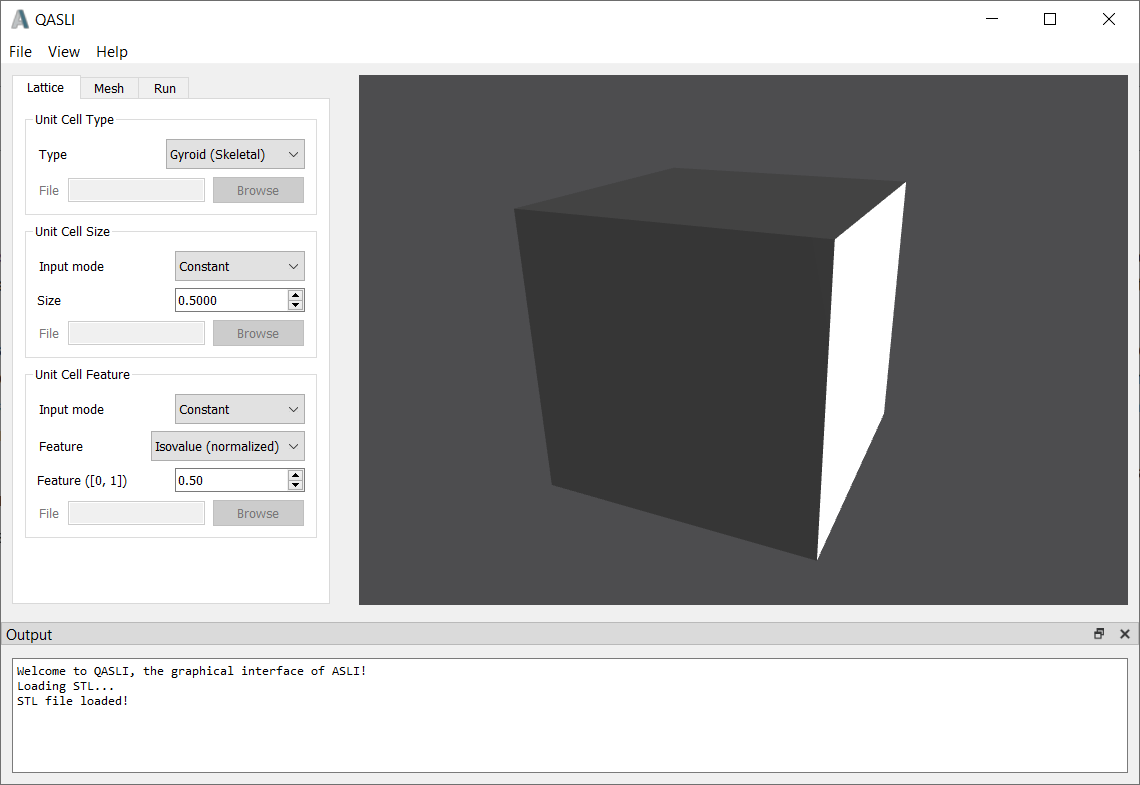
\includegraphics[width=\linewidth]{figures/gui.png}%
	
	\caption{QASLI, the graphical user interface of \asli{}.}
	\label{fig:gui}
\end{figure}

\subsection{Demo} \label{sec:demo}
\asli{} includes one demo problem. The files required for the demo are the \texttt{cube.stl} file, containing the $1\times1\times1$ cube shown in Fig. \ref{fig:cube}, and the \texttt{cube.tap}, \texttt{cube.sap} and \texttt{cube.fap} files, which contain the local type, size and feature (isovalue) specifications shown in Fig. \ref{fig:type_dp}-\subref{fig:feature_dp}. All four files can be found in the \texttt{inputs} folder of \asli{}.
\begin{figure}[htb]
	\centering
	\begin{subfigure}[t]{.225\textwidth}
		\centering
		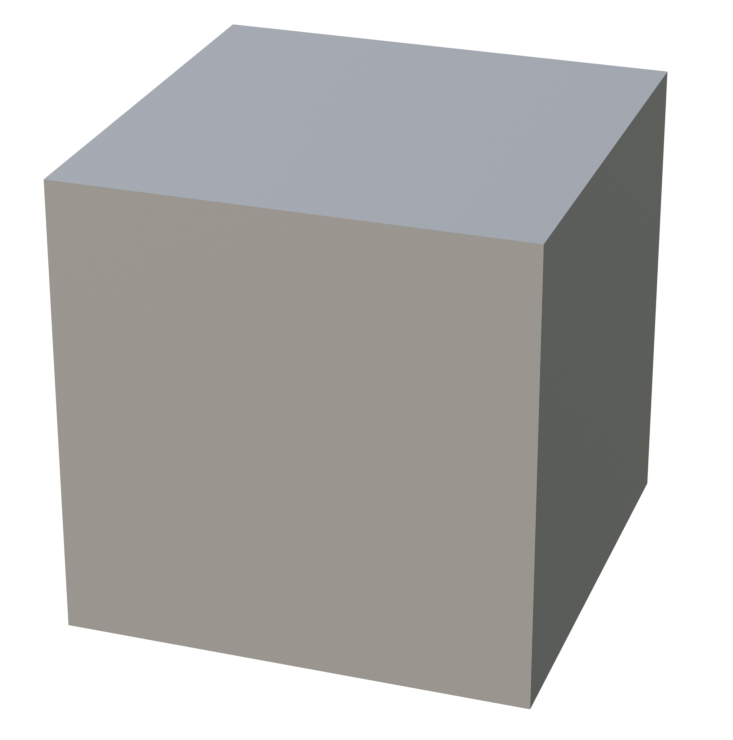
\includegraphics[width=\linewidth]{figures/cube.png}
		\caption{}\label{fig:cube}
	\end{subfigure}\hspace{1.0em}%
	\begin{subfigure}[t]{.225\textwidth}
		\centering
		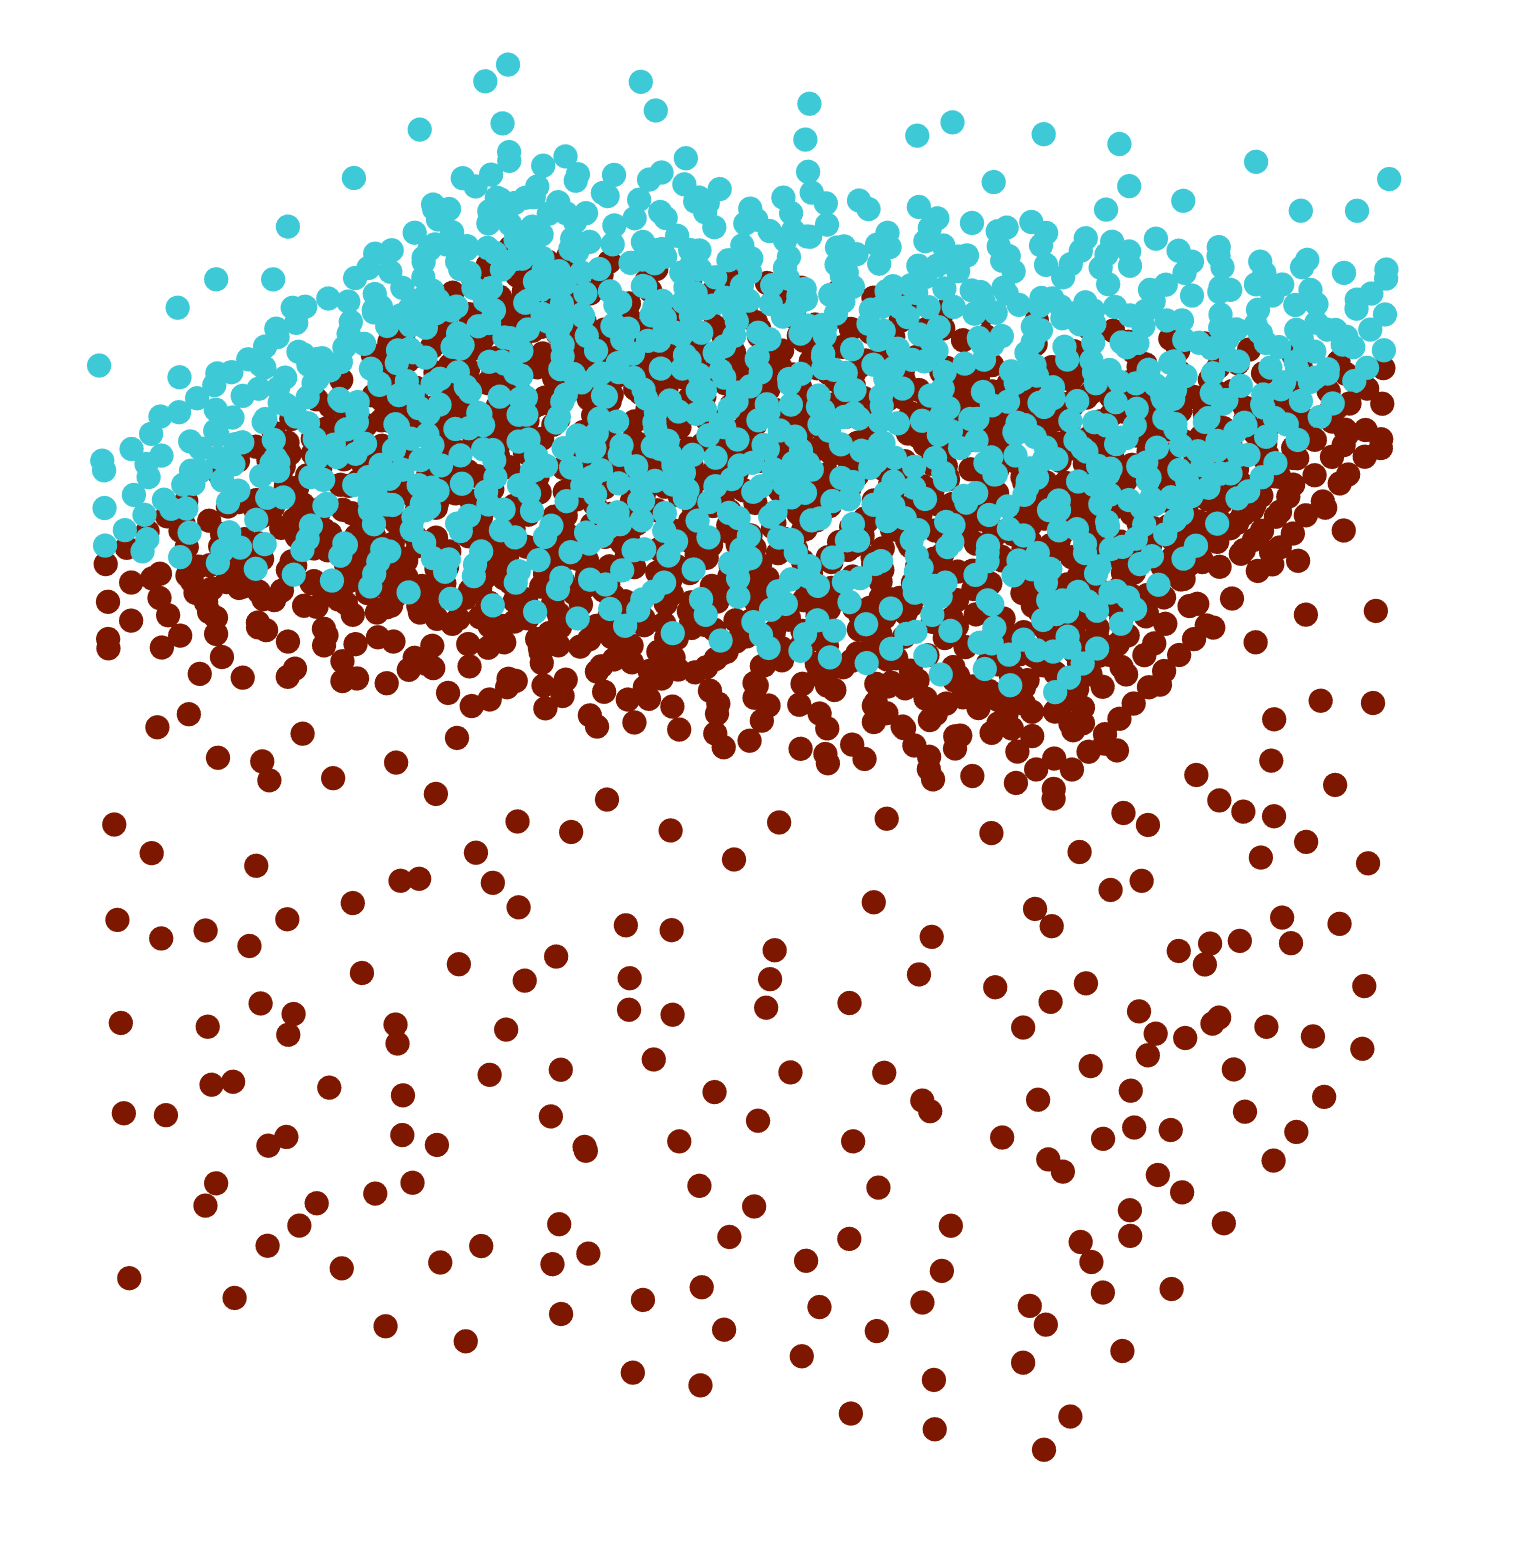
\includegraphics[width=\linewidth]{figures/cube_type_dp.png}
		\caption{}\label{fig:type_dp}
	\end{subfigure}\hspace{1.0em}%
	\begin{subfigure}[t]{.225\textwidth}
		\centering
		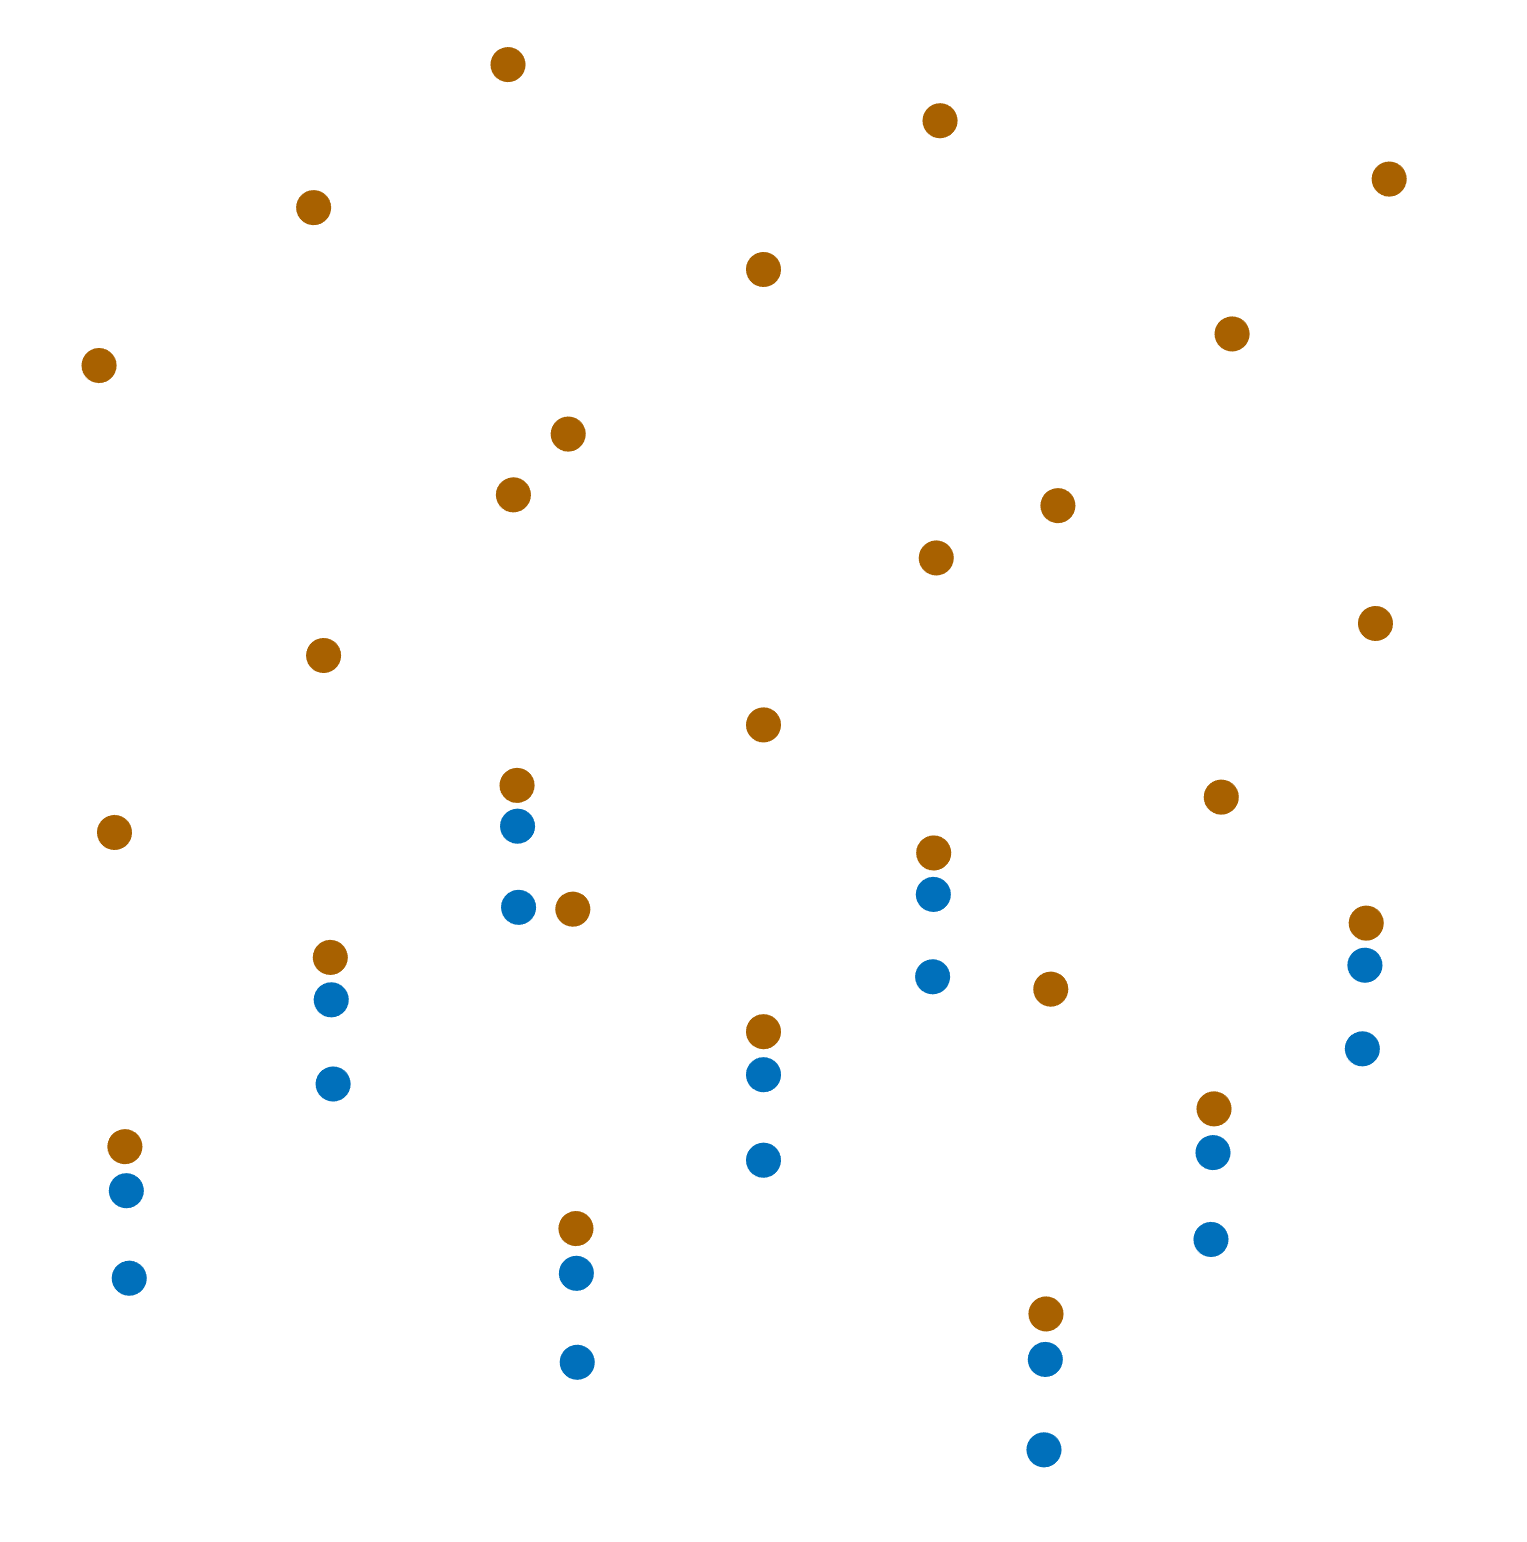
\includegraphics[width=\linewidth]{figures/cube_size_dp.png}
		\caption{}\label{fig:size_dp}
	\end{subfigure}\hspace{1.0em}%
	\begin{subfigure}[t]{.225\textwidth}
		\centering
		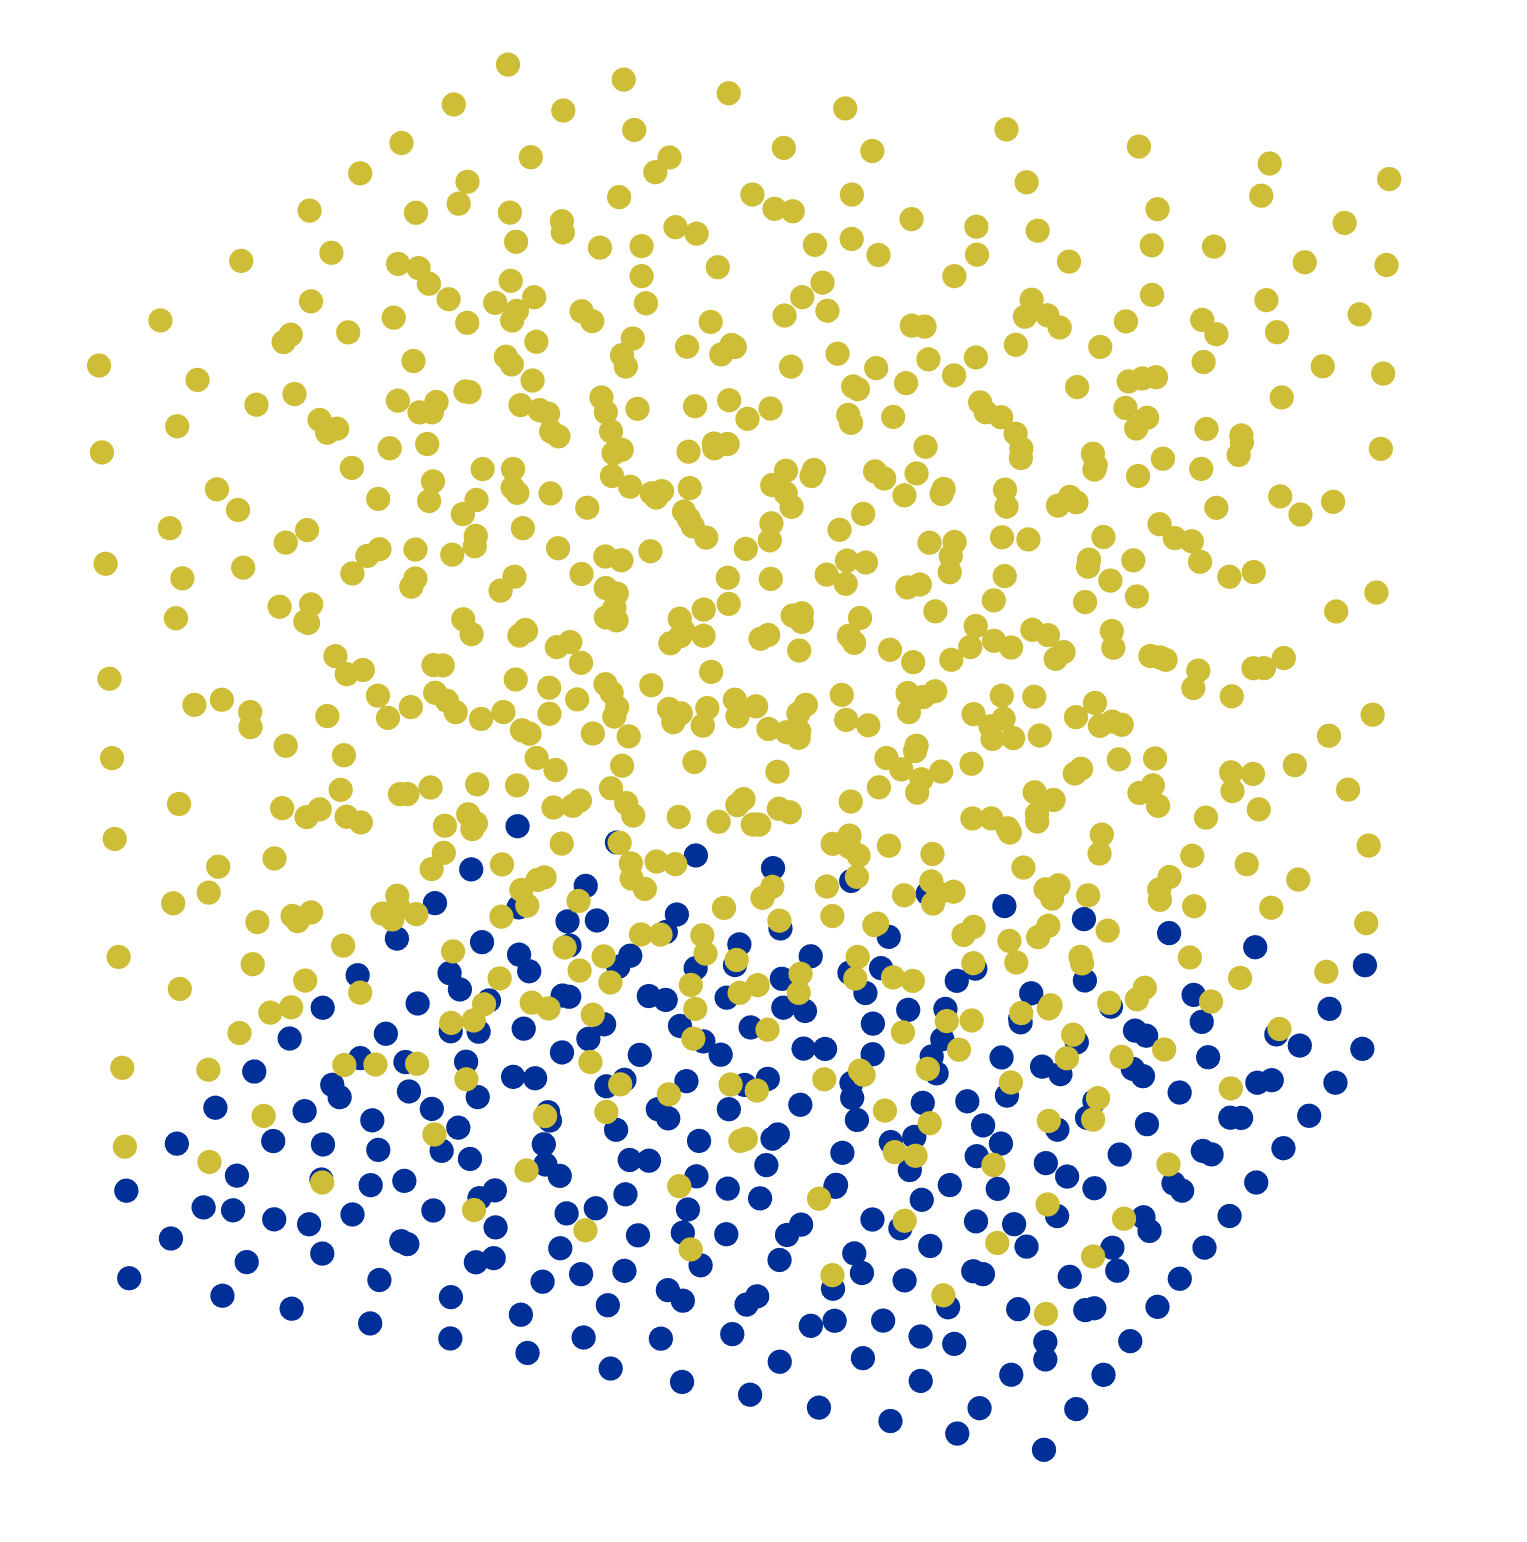
\includegraphics[width=\linewidth]{figures/cube_feature_dp.png}
		\caption{}\label{fig:feature_dp}
	\end{subfigure}%

	\caption{Input files of the demo problem (a) input geometry, (b) type at point data [\mycirc[myColorD] sheet-gyroid \mycirc[myColorA] strut-gyroid], (c) size at point data [\mycirc[myColorB] 0.25 \mycirc[myColorE] 0.5] and (d) feature at point data (isovalue) [\mycirc[myColorC] 0.35 \mycirc[myColorF] 1].}
	\label{fig:demo}
\end{figure}

The demo files allow users to create a cube with constant infill (Fig. \ref{fig:constant}) or a cube with a functionally graded infill that can be hybrid, pseudo-periodic and/or heterogeneous (Fig. \ref{fig:type}-\subref{fig:mixed}).
\begin{figure}[htb]
	\sbox0{\begin{subfigure}[t]{.225\linewidth}
			\centering
			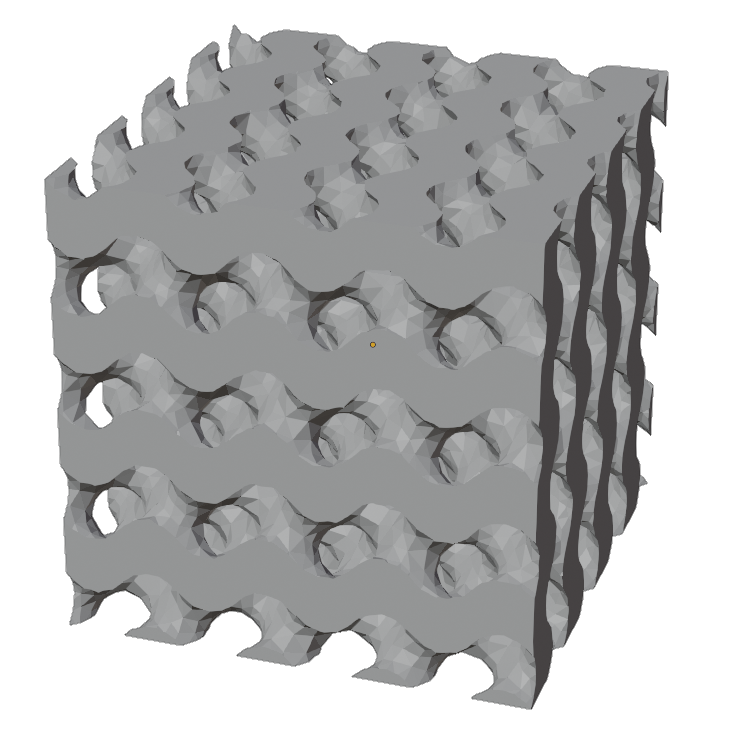
\includegraphics[width=\linewidth]{figures/cube_standart.png}
			\caption{}\label{fig:constant}
	\end{subfigure}}
	\sbox1{\begin{subfigure}[t]{.225\linewidth}
			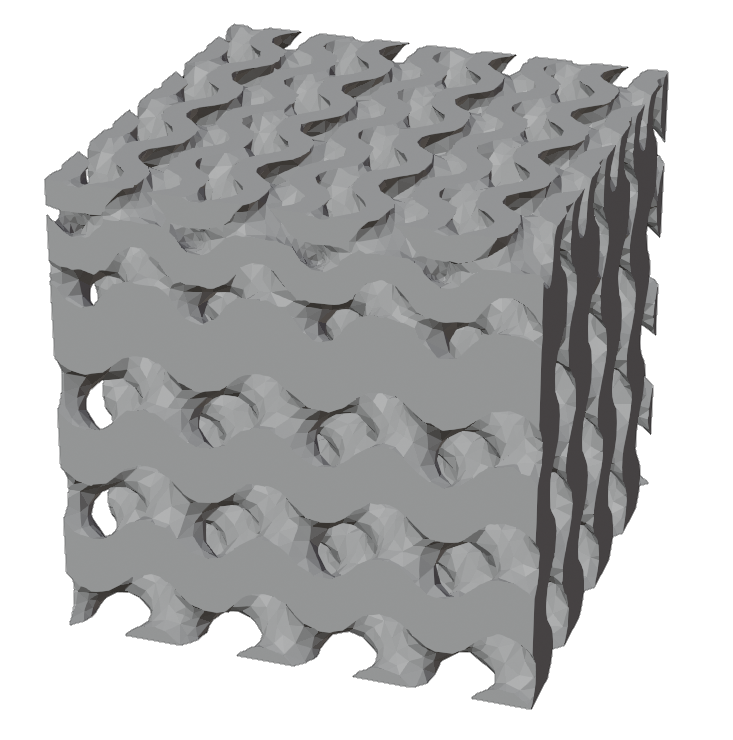
\includegraphics[width=\linewidth]{figures/cube_type.png}
			\caption{}\label{fig:type}
	\end{subfigure}}
	\sbox2{\begin{subfigure}[t]{.225\linewidth}
			\centering
			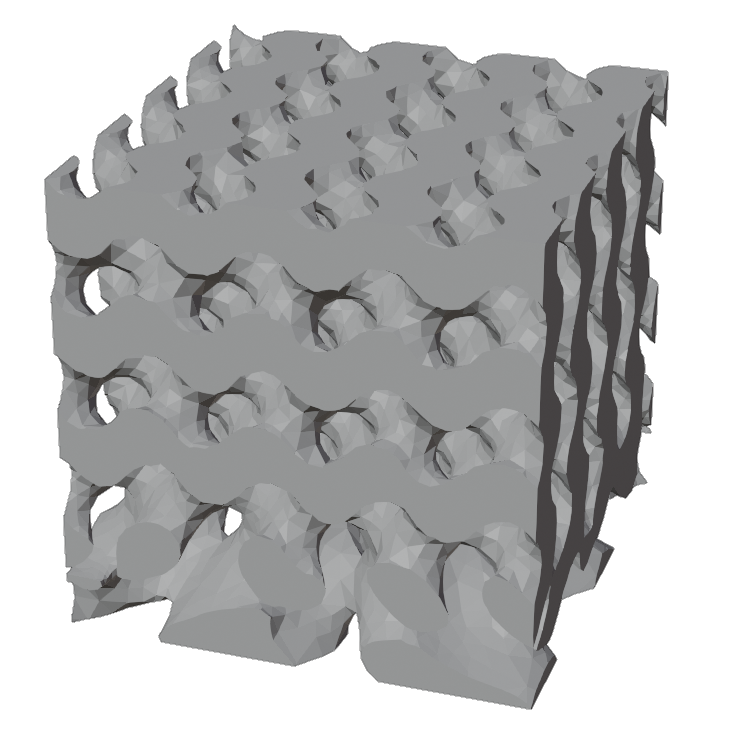
\includegraphics[width=\linewidth]{figures/cube_size.png}
			\caption{}\label{fig:size}
	\end{subfigure}}
	\sbox3{\begin{subfigure}[t]{.225\linewidth}
			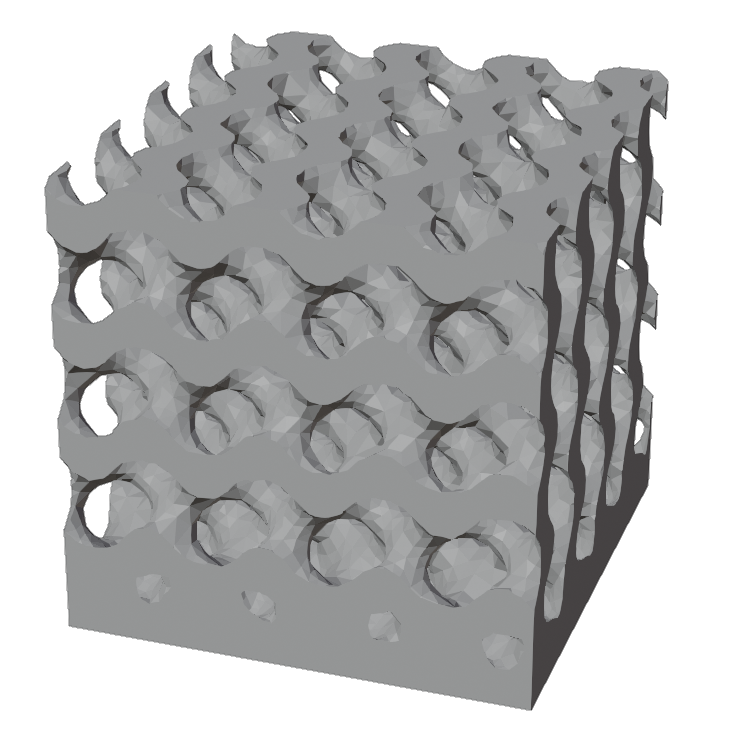
\includegraphics[width=\linewidth]{figures/cube_feature.png}
			\caption{}\label{fig:feature}
	\end{subfigure}}
	\sbox4{\begin{subfigure}[t]{.5\linewidth}
			\centering
			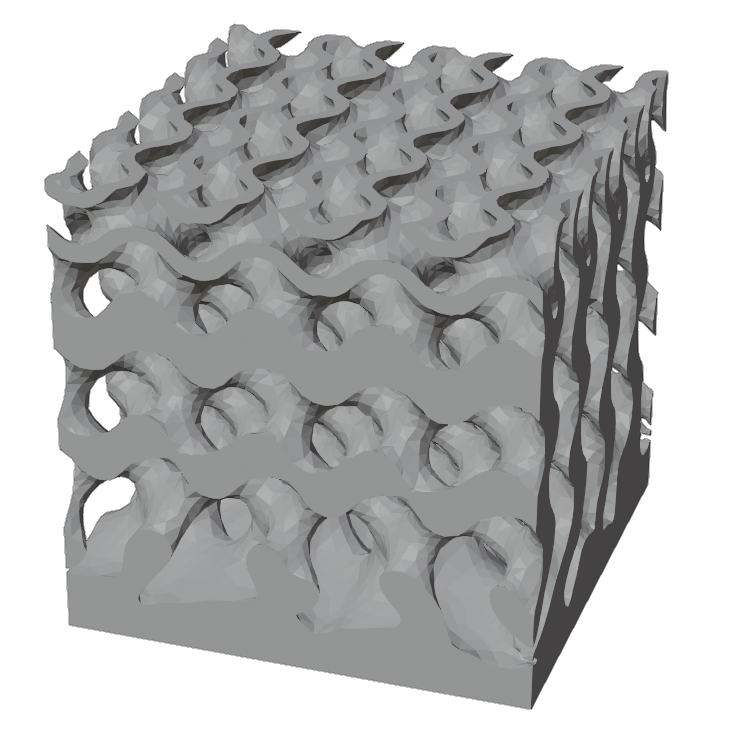
\includegraphics[width=\linewidth]{figures/cube_mixed.png}
			\caption{}\label{fig:mixed}
	\end{subfigure}}
	
	\centering
	\begin{minipage}{.5\textwidth}
		\usebox0\hfil \usebox1
		\usebox2\hfil \usebox3
	\end{minipage}%
	\begin{minipage}{.5\textwidth}
		\usebox4
	\end{minipage}
	
	\caption{$1\times1\times1$ cube with an (a) constant infill, (b) hybrid infill, (c) pseudo-periodic infill, (d) heterogeneous infill and (e) hybrid pseudo-periodic heterogeneous infill.}
	\label{fig:demo results}
\end{figure}

\subsubsection{Running the demo making use of the configuration file} \label{sec:demo config}
To run the demo problem using the configuration file start by opening the unedited \texttt{config.yml} file provided with a text editor and modify the parameters specified below depending on the infill you would like to obtain.
\begin{enumerate}[label=\alph*)]
	\item Constant infill (Fig. \ref{fig:constant})
	\begin{itemize}
		\item Set {\tt lt\_size} to {\tt 0.25}
	\end{itemize}	
	\item Hybrid infill (Fig. \ref{fig:type})
	\begin{itemize}
		\item Set {\tt tap} to {\tt inputs/cube.tap}
		\item Set {\tt lt\_type} {\tt to hybrid}
		\item Set {\tt lt\_size} {\tt to 0.25}
	\end{itemize}
	\item Pseudo-periodic infill (Fig. \ref{fig:size})
	\begin{itemize}
		\item Set {\tt sap} to {\tt inputs/cube.sap}
		\item Set {\tt lt\_size} to {\tt 0}
	\end{itemize}
	\item Heterogeneous infill (Fig. \ref{fig:feature})
	\begin{itemize}
		\item Set {\tt fap} to {\tt inputs/cube.fap}
		\item Set {\tt lt\_size} to {\tt 0.25}
		\item Set {\tt lt\_feature\_val} to {\tt 0}
	\end{itemize}
	\item Hybrid pseudo-periodic heterogeneous infill  (Fig. \ref{fig:mixed})
	\begin{itemize}
		\item Set {\tt tap} to {\tt inputs/cube.tap}
		\item Set {\tt sap} to {\tt inputs/cube.sap}
		\item Set {\tt fap} to {\tt inputs/cube.fap}
		\item Set {\tt lt\_type} to {\tt hybrid}
		\item Set {\tt lt\_size} to {\tt 0}
		\item Set {\tt lt\_feature\_val} to {\tt 0}
	\end{itemize}
\end{enumerate}

Save the modifications made and execute \asli{} by calling \verb|./ASLI config.yml| if using Linux or \verb|ASLI.exe config.yml| if using windows. The generated lattice will be stored as an \texttt{.stl} file in the outputs folder.

\subsubsection{Running the demo making use of the GUI} \label{sec:demo GUI}
To run the demo using the GUI the first step, after opening \qasli{}, is to load the \texttt{.stl} file containing the geometry to be provided of an infill. To do so go to \menu{File > Load Surface (.stl)}, open the folder \texttt{inputs}, select the file named \texttt{cube.stl} and click \menu{Open}.

Next, set the lattice and mesh parameters depending on the infill you would like to obtain following the instructions below. %. ???The steps required to obtain the infills for all five scenarios shown in Fig. \ref{fig:demo results}\subref{fig:constant}-\subref{fig:mixed} are listed bellow.

\begin{enumerate}[label=\alph*)]
	\item Constant infill (Fig. \ref{fig:constant})
		\begin{enumerate}[label=\arabic*.]
			\item Set \tabmenu{Lattice > Unit Cell Size > Size} to {\tt 0.25}
		\end{enumerate}	
	\item Hybrid infill (Fig. \ref{fig:type})
	\begin{enumerate}[label=\arabic*.]
		\item Set \tabmenu{Lattice > Unit Cell Type > Type} to `\textit{From file}'
		\item Click on the corresponding \menu{Browse} button, navigate to the \texttt{inputs} folder, select the file \texttt{cube.tap} and click  \menu{Open}.
		\item Set \tabmenu{Lattice > Unit Cell Size > Size} to {\tt 0.25}
		\item Set  \tabmenu{Mesh > Mesh Engine > Mesher} to `\textit{CGAL}'
	\end{enumerate}
	\item Pseudo-periodic infill (Fig. \ref{fig:size})
	\begin{enumerate}[label=\arabic*.]
		\item Set \tabmenu{Lattice > Unit Cell Size > Input mode} to `\textit{From file}'
		\item Click on the corresponding \menu{Browse} button, navigate to the \texttt{inputs} folder, select the file \texttt{cube.sap} and click  \menu{Open}.
		\item Set  \tabmenu{Mesh > Mesh Engine > Mesher} to `\textit{CGAL}'
	\end{enumerate}
	\item Heterogeneous infill (Fig. \ref{fig:feature})
	\begin{enumerate}[label=\arabic*.]
		\item Set \tabmenu{Lattice > Unit Cell Size > Size} to {\tt 0.25}
		\item Set \tabmenu{Lattice > Unit Cell Feature > Input mode} to `\textit{From file}'
		\item Click on the corresponding \menu{Browse} button, navigate to the \texttt{inputs} folder, select the file \texttt{cube.fap} and click  \menu{Open}.
		\item Set \tabmenu{Mesh > Mesh Engine > Mesher} to `\textit{CGAL}'
	\end{enumerate}
	\item Hybrid pseudo-periodic heterogeneous infill  (Fig. \ref{fig:mixed})
	\begin{enumerate}[label=\arabic*.]
		\item Set \tabmenu{Lattice > Unit Cell Type > Type} to `\textit{From file}'
		\item Click on the corresponding \menu{Browse} button, navigate to the \texttt{inputs} folder, select the file \texttt{cube.tap} and click  \menu{Open}.
		\item Set \tabmenu{Lattice > Unit Cell Size > Input mode} to `\textit{From file}`
		\item Click on the corresponding \menu{Browse} button, navigate to the \texttt{inputs} folder, select the file \texttt{cube.sap} and click  \menu{Open}.
		\item Set \tabmenu{Lattice > Unit Cell Feature > Input mode} to `\textit{From file}'
		\item Click on the corresponding \menu{Browse} button, navigate to the \texttt{inputs} folder, select the file \texttt{cube.fap} and click  \menu{Open}.
		\item Set  \tabmenu{Lattice > Mesh Engine > Mesher} to `\textit{CGAL}'
	\end{enumerate}
\end{enumerate}

Finally, go to the \tabmenu{Run} tab and click \menu{Run}. Once finished you will be notified, dismiss the notice by clicking on \menu{Ok}. The generated lattice will be displayed automatically in the viewer and stored as an \texttt{.stl} file in the outputs folder.

\subsection{Other examples} \label{sec:use cases}
A few examples that showcase \asli{} capabilities are shown in Fig. \ref{fig:examples}.

\begin{figure}[htb]
	\centering
	\sbox0{\begin{subfigure}[t]{.35\linewidth}
		\centering
		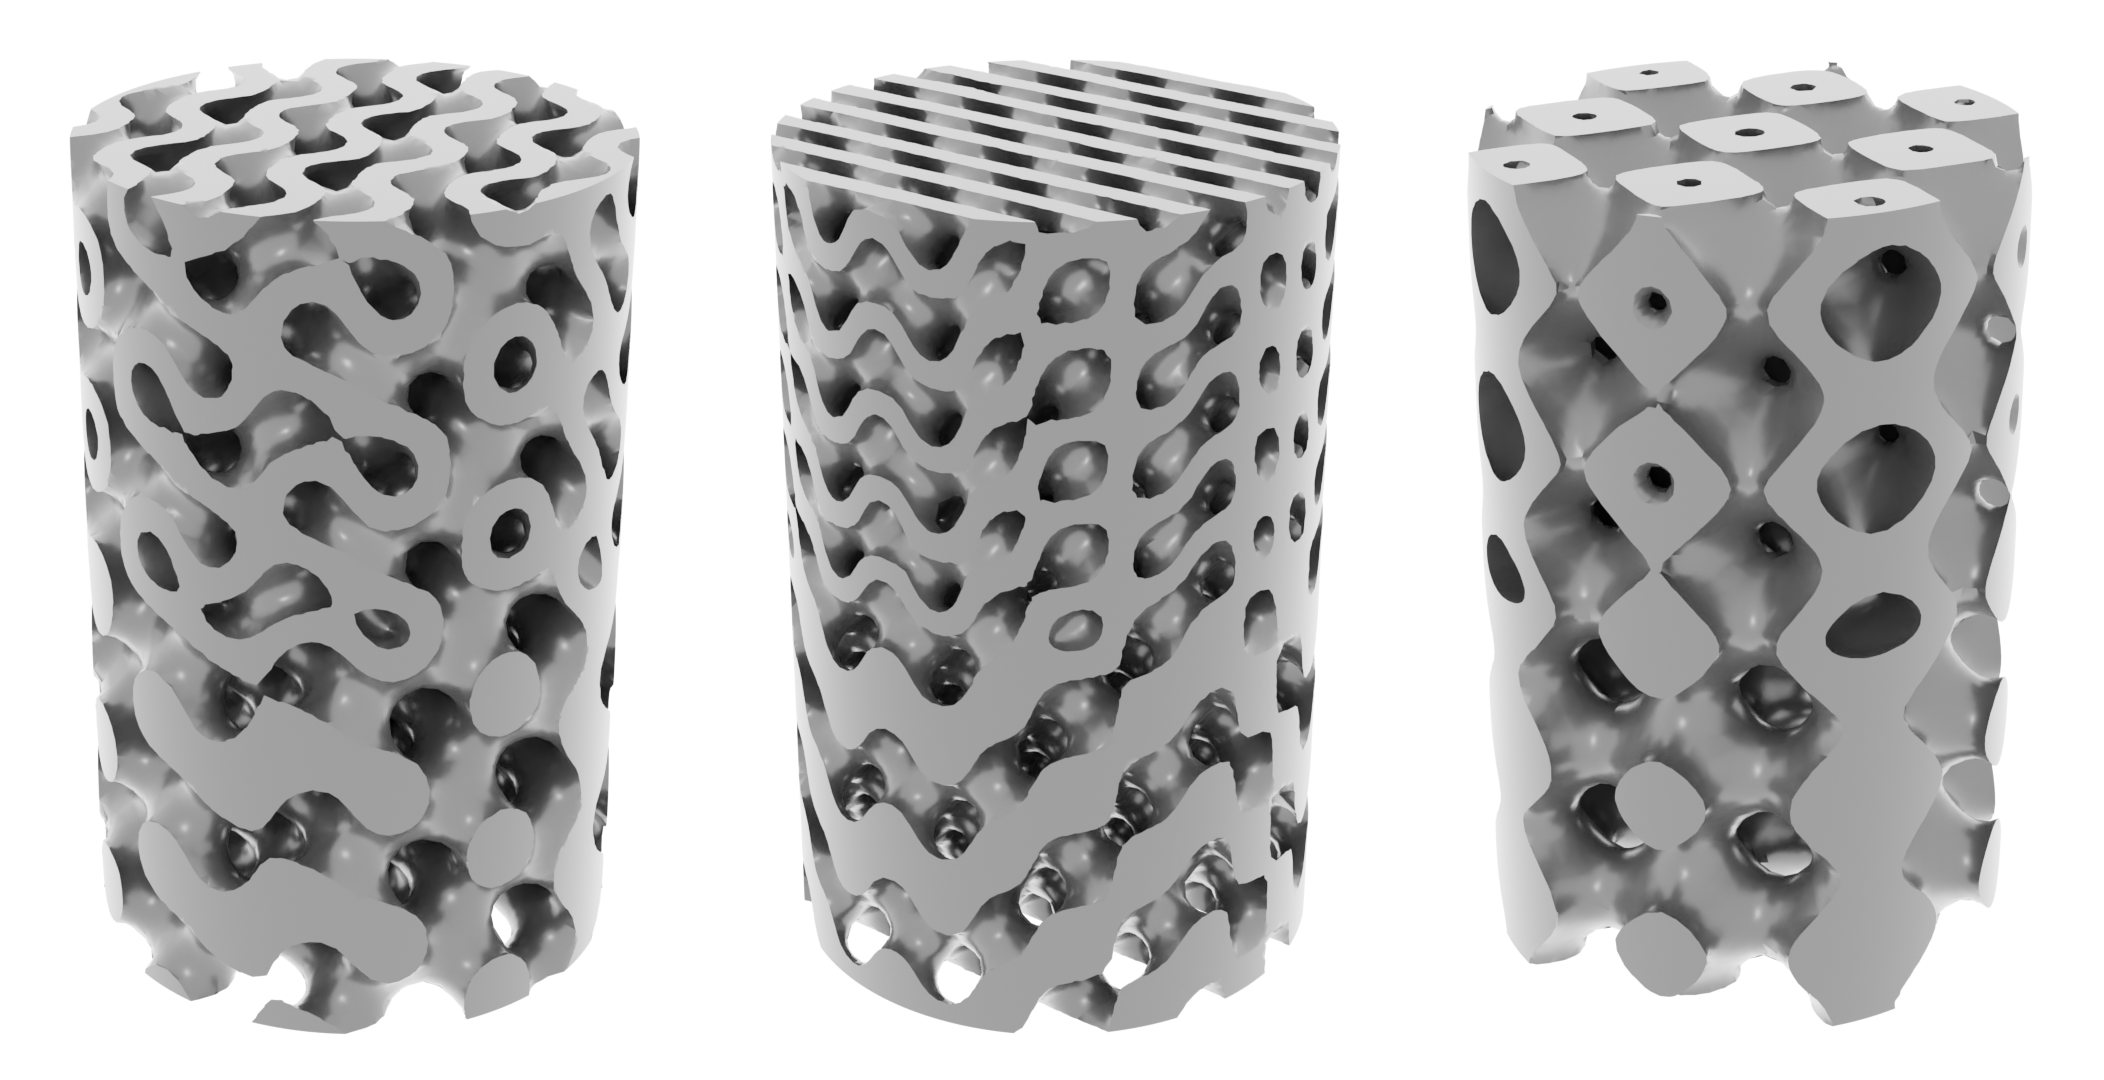
\includegraphics[width=\linewidth]{figures/Sample-S5VF0p5.png}
		\caption{}\label{fig:cylinders}
	\end{subfigure}}
	\sbox1{\begin{subfigure}[t]{.35\linewidth}
		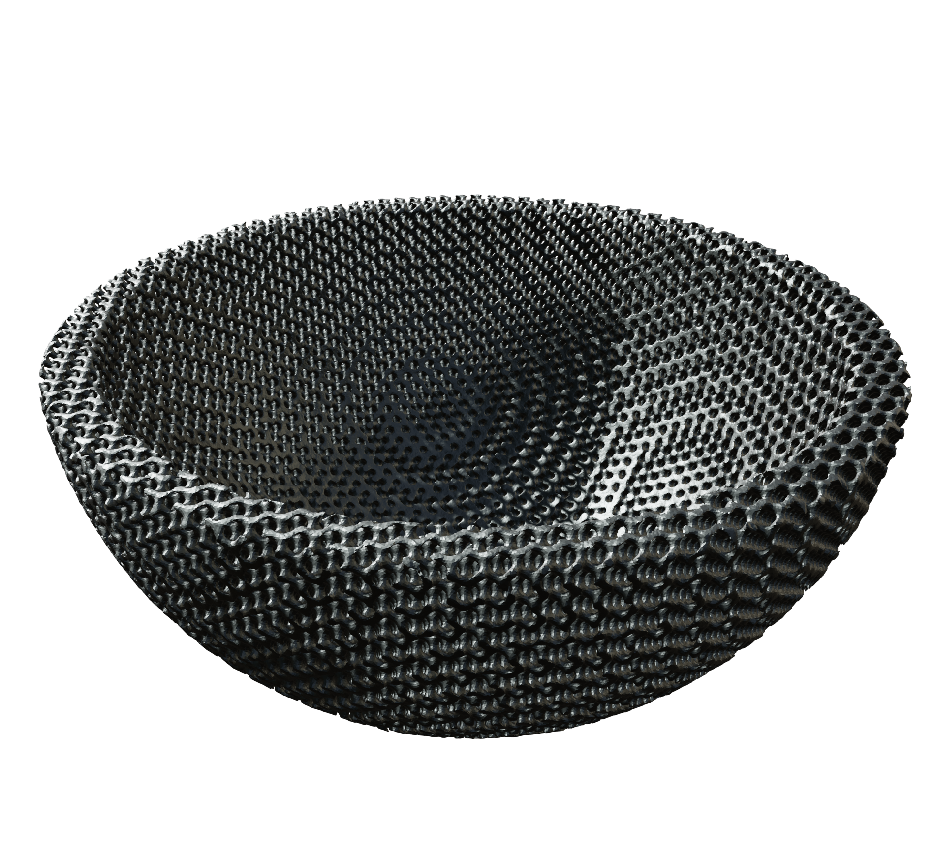
\includegraphics[width=\linewidth]{figures/acetabular_implant.png}
		\caption{}\label{fig:acetabular implant}
	\end{subfigure}}
	\sbox2{\begin{subfigure}[t]{.58\linewidth}
		\centering
		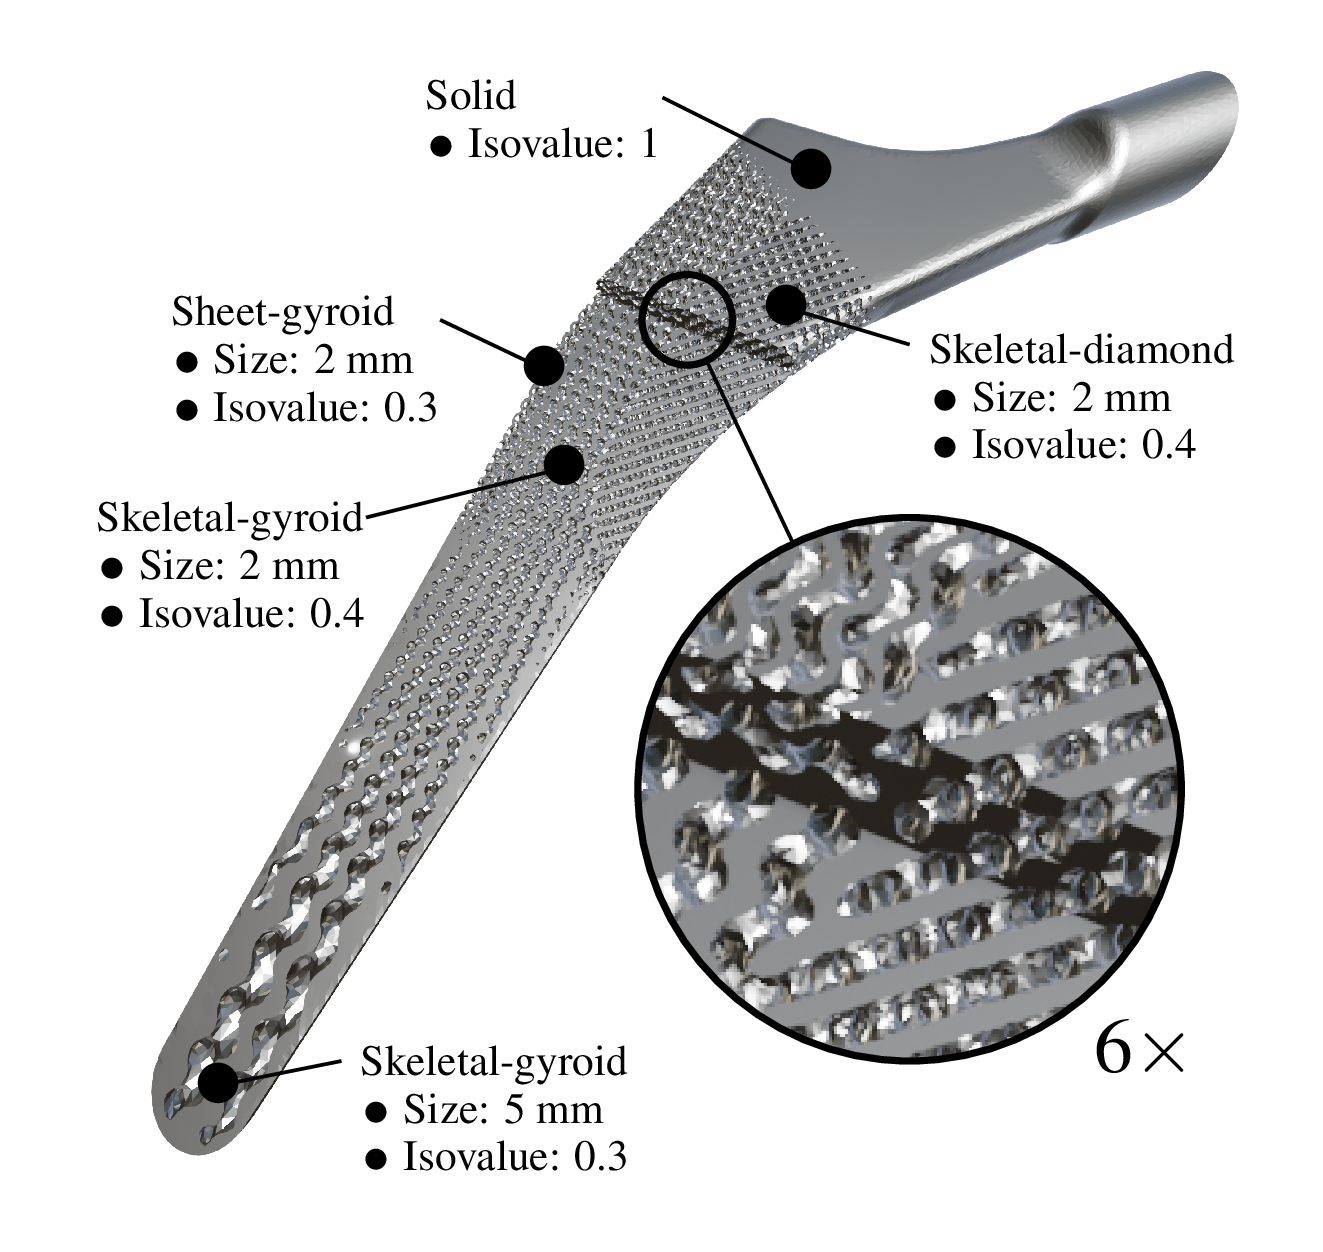
\includegraphics[width=\linewidth]{figures/femoral_implant.png}
		\caption{}\label{fig:femoral implat}
	\end{subfigure}}
	
	\centering
	\begin{minipage}{.35\textwidth}
		\usebox0 \\
		\usebox1
	\end{minipage}%
	\begin{minipage}{.58\textwidth}
		\usebox2
	\end{minipage}

	\caption{Examples of lattice structures generated with \asli{}: (a) functionally graded cylinder test samples, (b) functionally graded acetabular cup and (c) functionally graded femoral implant with stem cut in half to show internal structure.}
	\label{fig:examples}
\end{figure}
	
	% Support
	\section{Support} \label{sec:questions-and-answers}
If you have questions not addressed in this manual, there are a number of resources listed below you can use.

\begin{itemize}
\item You can create a post on \href{https://stackoverflow.com/questions/tagged/ASLI}{stackoverflow} with the tag `\href{https://stackoverflow.com/questions/tagged/ASLI}{ASLI}'.

\item You can report bugs using \asli{} issue tracker on \href{https://github.com/tpms-lattice/ASLI/issues}{GitHub}. You are also welcome to use the issue tracker to ask questions or post suggestions.

\item If you have specific questions about \asli{} that are not suitable for public and archived mailing lists you can contact us at \url{asli@kuleuven.be}.
  
\item \asli{} relies on \href{https://www.cgal.org/}{CGAL} and \href{https://www.mmgtools.org/}{MMG} in order to discretize the scaffolds. If you have specific questions about CGAL or MMG, you can contact their communities at \url{https://www.cgal.org/support.html} and \url{https://forum.mmgtools.org}.
\end{itemize}

	\clearpage
	
	% Appendices
	\appendix
	\section*{Appendix A: Input parameters} \label{sec:parameters}
\addcontentsline{toc}{section}{Appendix A: Input parameters}
\setcounter{section}{1}
\renewcommand{\thesection}{\Alph{section}}

\asli{} requires multiple parameters to be specified by the user. A description of all input parameters is found below. Some of the parameters have default values. These default values work well for many use cases and are therefore considered a good starting point. In the description of the input parameters there is also a ``Standard/Advanced'' label included. ``Advanced'' parameters are only required for specific cases and be can be ignored otherwise. For convenience all input parameters are indexed in the Section ``\hyperref[sec:index inputs full]{Index of input parameters}'' found at the end of the manual.

\subsection{Input/output files} \label{parameters:files}
\begin{itemize}
	% stl
	\item {\it Parameter name:} {\tt stl}
	\phantomsection
	\label{parameters:stl}
	
	\index[prmindex]{stl}
	\index[prmindexfull]{IO files!stl file}
	
	{\it Default:} Should be provided
	
	{\it Description:} [Standard] STL file containing the object to be provided of an infill.
	
	{\it Possible values:} String value
	
	% tap
	\item {\it Parameter name:} {\tt tap}
	\phantomsection
	\label{parameters:tap}
	
	\index[prmindex]{tap}
	\index[prmindexfull]{IO files!tap file}
	
	{\it Default:} Should be provided
	
	{\it Description:} [Standard] Type at point file containing local unit cell type specifications.
	
	{\it Possible values:} String value
	
	% sap
	\item {\it Parameter name:} {\tt sap}
	\phantomsection
	\label{parameters:sap}
	
	\index[prmindex]{sap}
	\index[prmindexfull]{IO files!sap file}
	
	{\it Default:} Should be provided
	
	{\it Description:} [Standard] Size at point file containing local unit cell size specifications.
	
	{\it Possible values:} String value
	
	% fap
	\item {\it Parameter name:} {\tt fap}
	\phantomsection
	\label{parameters:fap}
	
	\index[prmindex]{fap}
	\index[prmindexfull]{IO files!fap file}
	
	{\it Default:} Should be provided
	
	{\it Description:} [Standard] Feature at point file containing local unit cell feature specifications.
	
	{\it Possible values:} String value
	
	% output
	\item {\it Parameter name:} {\tt output}
	\phantomsection
	\label{parameters:output}
	
	\index[prmindex]{output}
	\index[prmindexfull]{IO files!output location}
	
	{\it Default:} ./outputs/
	
	{\it Description:} [Standard] Location were the output file(s) will be stored.
	
	{\it Possible values:} String value
\end{itemize}

\subsection{Lattice parameters} \label{parameters:lattice}
\begin{itemize}
	% lt_type
	\item {\it Parameter name:} {\tt lt\_type}
	\phantomsection
	\label{parameters:lt_type}

	\index[prmindex]{lt\_type}
	\index[prmindexfull]{Lattice!lattice type}
	
	{\it Default:} Should be provided
	
	{\it Description:} [Standard] Parameter specifying the unit cell type, i.e. {\it gyroid}, {\it sheet\_gyroid}, {\it diamond}, {\it sheet\_diamond}, {\it primitive}, {\it sheet\_primitive}, {\it IWP} or {\it sheet\_IWP}. To specify multiple unit cell types set to {\it hybrid} and provide a .tap file (see \hyperref[parameters:tap]{\tt tap} parameter).
	
	{\it Possible values:} String value
	
	% lt_type_filterRadius
	\item {\it Parameter name:} {\tt lt\_type\_filterRadius}
	\phantomsection
	\label{parameters:lt_type_filterRadius}
	
	\index[prmindex]{lt\_type\_filterRadius}
	\index[prmindexfull]{Lattice!filter radius}
	
	{\it Default:} 1.0
	
	{\it Description:} [Advanced] Radius specifying the size of hybrid regions. The radius scales automatically with local unit cell size. Only active if {\tt lt\_type} is set to {\it hybrid}.
	
	{\it Possible values:} Non-negative floating point number
	
	% lt_type_correctionFactor
	\item {\it Parameter name:} {\tt lt\_type\_correctionFactor}
	\phantomsection
	\label{parameters:lt_type_correctionFactor}
	
	\index[prmindex]{lt\_type\_correctionFactor}
	\index[prmindexfull]{Lattice!correction factor}
	
	{\it Default:} 0.25
	
	{\it Description:} [Advanced] Correction factor to compensate for the thinning effect of hybridization. Only active if {\tt lt\_type} is set to {\it hybrid}.
	
	{\it Possible values:} Non-negative floating point number
	
	% lt_size
	\item {\it Parameter name:} {\tt lt\_size}
	\phantomsection
	\label{parameters:lt_size}
	
	\index[prmindex]{lt\_size}
	\index[prmindexfull]{Lattice!size}
	
	{\it Default:} Should be provided
	
	{\it Description:} [Standard] Parameter specifying the unit cell size. Set to a value larger than 0 for a constant unit cell size. To prescribe a variable unit cell size set to 0 and provide a .sap file (see \hyperref[parameters:sap]{\tt sap} parameter).
	
	{\it Possible values:} Non-negative floating point number
	
	% lt_feature
	\item {\it Parameter name:} {\tt lt\_feature}
	\phantomsection
	\label{parameters:lt_feature}
	
	\index[prmindex]{lt\_feature}
	\index[prmindexfull]{Lattice!feature}
	
	{\it Default:} Should be provided
	
	{\it Description:} [Standard] Parameter specifying the unit cell feature that will be specified, i.e. {\it isovalue}, {\it volumeFraction}, {\it wallSize} or {\it poreSize}.
	
	{\it Possible values:} String value
	
	% lt_feature_val
	\item {\it Parameter name:} {\tt lt\_feature\_val}
	\phantomsection
	\label{parameters:lt_feature_val}
	
	\index[prmindex]{lt\_feature\_val}
	\index[prmindexfull]{Lattice!feature value}
	
	{\it Default:} Should be provided
	
	{\it Description:} [Standard] Parameter specifying the unit cell feature value. Set to a value larger than 0 for a constant feature value. To prescribe a variable feature value set to 0 and provide a .fap file (see \hyperref[parameters:fap]{\tt fap} parameter). If the feature value being provided is an isovalue, it should be specified as a normalized isovalue
	
	{\it Possible values:} Non-negative floating point number
	
	% lt_feature_mode
	\item {\it Parameter name:} {\tt lt\_feature\_mode}
	\phantomsection
	\label{parameters:lt_feature_mode}
	
	\index[prmindex]{lt\_feature\_mode}
	\index[prmindexfull]{Lattice!feature mode}
	
	{\it Default:} relative
	
	{\it Description:} [Advanced] Parameter specifying the feature size mode, i.e. {\it absolute} or {\it relative}. Only active if {\tt lt\_feature} is set to {\it wallSize} or {\it poreSize}. If set to relative, provide wall and pore sizes relative to a $1 \times 1 \times 1$ unit cell.
	
	{\it Possible values:} String value
\end{itemize}

\subsection{Mesh parameters} \label{parameters:mesh}
\begin{itemize}
	% me_mesher
	\item {\it Parameter name:} {\tt me\_mesher}
	\phantomsection
	\label{parameters:me_mesher}
	
	\index[prmindex]{me\_mesher}
	\index[prmindexfull]{Mesh!mesher}
	
	{\it Description:} [Standard] Parameter specifying the mesh library to use, i.e. {\it CGAL} or {\it MMG}.
	
	{\it Default:} Should be provided
	
	{\it Possible values:} String value
	
	% me_side
	\item {\it Parameter name:} {\tt me\_side}
	\phantomsection
	\label{parameters:me_side}
	
	\index[prmindex]{me\_side}
	\index[prmindexfull]{Mesh!side}
	
	{\it Default:} scaffold
	
	{\it Description:} [Advanced] Parameter specifying the side of the scaffold to discretize, i.e. {\it scaffold} or {\it void}.
	
	{\it Possible values:} String value
	
	% me_volumeMesh
	\item {\it Parameter name:} {\tt me\_volumeMesh}
	\phantomsection
	\label{parameters:me_volumeMesh}
	
	\index[prmindex]{me\_volumeMesh}
	\index[prmindexfull]{Mesh!volume mesh}
	
	{\it Default:} FALSE
	
	{\it Description:} [Advanced] Parameter specifying if the volume should also be discretized. Set to TRUE to discretize the volume, otherwise only the surface mesh will be generated.
	
	{\it Possible values:} Boolean value (TRUE or FALSE) 
	
	% me_nThreads
	\item {\it Parameter name:} {\tt me\_nThreads}
	\phantomsection
	\label{parameters:me_nThreads}
	
	\index[prmindex]{me\_nThreads}
	\index[prmindexfull]{Mesh!number of threads}
	
	{\it Default:} 1
	
	{\it Description:} [Standard] Number of threads to use. (Parallel mode is currently only available when {\tt me\_mesher} is set to CGAL)
	
	{\it Possible values:} Positive integer value
\end{itemize}

% CGAL parameters
\subsubsection{CGAL specific parameters} \label{parameters:cgal}
\begin{itemize}
	% me_facetAngle
	\item {\it Parameter name:} {\tt me\_facetAngle}
	\phantomsection
	\label{parameters:me_facetAngle}
	
	\index[prmindex]{me\_facetAngle}
	\index[prmindexfull]{Mesh!CGAL!facet angle}
	
	{\it Default:} 30
	
	{\it Description:} [Standard] Surface facet shape, i.e. lower bound for the surface facets angle in degrees.
	
	{\it Possible values:} Positive floating point number 
	
	% me_facetSize
	\item {\it Parameter name:} {\tt me\_facetSize}
	\phantomsection
	\label{parameters:me_facetSize}
	
	\index[prmindex]{me\_facetSize}
	\index[prmindexfull]{Mesh!CGAL!facet size}
	
	{\it Default:} [The local unit cell size]
	
	{\it Description:} [Standard] Surface facet size, i.e. upper bound for the radii of surface Delaunay balls. Scales with unit cell size.
	
	{\it Possible values:} Positive floating point number 
	
	% me_facetDistance
	\item {\it Parameter name:} {\tt me\_facetDistance}
	\phantomsection
	\label{parameters:me_facetDistance}
	
	\index[prmindex]{me\_facetDistance}
	\index[prmindexfull]{Mesh!CGAL!facet distance}
	
	{\it Default:} Should be provided
	
	{\it Description:} [Standard] Surface approximation error, i.e. upper bound for the distance between the circumcenter of a surface facet and the center of the surface Delaunay ball of this facet. Scales with the unit cell size.
	
	{\it Possible values:} Positive floating point number 
	
	% me_cellRadiusEdgeRatio
	\item {\it Parameter name:} {\tt me\_cellRadiusEdgeRatio}
	\phantomsection
	\label{parameters:me_cellRadiusEdgeRatio}
	
	\index[prmindex]{me\_cellRadiusEdgeRatio}
	\index[prmindexfull]{Mesh!CGAL!cell radius edge ratio}
	
	{\it Default:} 3.0
	
	{\it Description:} [Standard] Tetrahedron shape quality measure, i.e. upper bound for the ratio between the circumradius of a mesh tetrahedron and its shortest edge. Only active if {\tt  me\_volumeMesh} is set to TRUE.
	
	{\it Possible values:} Positive floating point number larger than 2
	
	% me_cellSize
	\item {\it Parameter name:} {\tt me\_cellSize}
	\phantomsection
	\label{parameters:me_cellSize}
	
	\index[prmindex]{me\_cellSize}
	\index[prmindexfull]{Mesh!CGAL!cell size}
	
	{\it Default:} [The local wall size]
	
	{\it Description:} [Standard] Tetrahedra size, i.e. upper bound on the circumradii of the mesh tetrahedra. Only active if {\tt  me\_volumeMesh} is set to TRUE. Scales with wall size.
		
	{\it Possible values:} Positive integer number 
	
	% me_preserveEdges
	\item {\it Parameter name:} {\tt me\_preserveEdges}
	\phantomsection
	\label{parameters:me_preserveEdges}
	
	\index[prmindex]{me\_preserveEdges}
	\index[prmindexfull]{Mesh!CGAL!preserve edges}
	
	{\it Default:} TRUE
	
	{\it Description:} [Advanced] Set to TRUE to preserve the edges, otherwise set to FALSE.
	
	{\it Possible values:} Boolean value (TRUE or FALSE)
	
	% me_poissonOffset
	\item {\it Parameter name:} {\tt me\_poissonOffset}
	\phantomsection
	\label{parameters:me_poissonOffset}
	
	\index[prmindex]{me\_poissonOffset}
	\index[prmindexfull]{Mesh!CGAL!poisson offset}
	
	{\it Default:} 0.5
	
	{\it Description:} [Advanced] Poisson reconstruction offset. Scales with largest unit cell size in the design. Only active if {\tt me\_preserveEdges} is set to TRUE.
	
	{\it Possible values:} Positive floating point number larger or equal than 0.1
\end{itemize}

% MMG parameters
\subsubsection{Mmg specific parameters} \label{parameters:mmg}
\begin{itemize}
	% me_hvol
	\item {\it Parameter name:} {\tt me\_hvol}
	\phantomsection
	\label{parameters:me_hvol}
	
	\index[prmindex]{me\_hvol}
	\index[prmindexfull]{Mesh!MMG!hvol}
	
	{\it Default:} 1.5
	
	{\it Description:} [Standard] Maximum volume constraint of the intermediate TetGen mesh. Scales with the the smallest unit cell size in the design.
	
	{\it Possible values:} Positive floating point number
	
	% me_hinitial
	\item {\it Parameter name:} {\tt me\_hinitial}
	\phantomsection
	\label{parameters:me_hinitial}
	
	\index[prmindex]{me\_hinitial}
	\index[prmindexfull]{Mesh!MMG!hinitial}
	
	{\it Default:} 0.36
	
	{\it Description:} [Standard] Mesh size of the mesh used to compute the level-set. Scales with the smallest feature size.
	
	{\it Possible values:} Positive floating point number
	
	% me_hmin
	\item {\it Parameter name:} {\tt me\_hmin}
	\phantomsection
	\label{parameters:me_hmin}
	
	\index[prmindex]{me\_hmin}
	\index[prmindexfull]{Mesh!MMG!hmin}
	
	{\it Default:} [Inactive]
	
	{\it Description:} [Standard] Minimum edge size. Scales with the smallest feature size in the design.
	
	{\it Possible values:} Non-negative floating point number
	
	% me_hmax
	\item {\it Parameter name:} {\tt me\_hmax}
	\phantomsection
	\label{parameters:me_hmax}
	
	\index[prmindex]{me\_hmax}
	\index[prmindexfull]{Mesh!MMG!hmax}
	
	{\it Default:} [Inactive]
	
	{\it Description:} [Advanced] Maximum edge size. Scales with the largest feature size in the design.
	
	{\it Possible values:} Non-negative floating point number
	
	% me_hausd
	\item {\it Parameter name:} {\tt me\_hausd}
	\phantomsection
	\label{parameters:me_hausd}
	
	\index[prmindex]{me\_hausd}
	\index[prmindexfull]{Mesh!MMG!hausd}
	
	{\it Default:} Should be provided
	
	{\it Description:} [Advanced] Maximal Hausdorff distance for the boundaries approximation. Scales with the mean feature size.
	
	{\it Possible values:} Positive floating point number
	
	% me_hgrad
	\item {\it Parameter name:} {\tt me\_hgrad}
	\phantomsection
	\label{parameters:me_hgrad}
	
	\index[prmindex]{me\_hgrad}
	\index[prmindexfull]{Mesh!MMG!hgrad}
	
	{\it Default:} 1.3
	
	{\it Description:} [Advanced] Gradation value. Only active if {\tt  me\_volumeMesh} is set to TRUE.
	
	{\it Possible values:} Positive floating point number
	
\end{itemize}

	\clearpage
	
	% Index of input parameters
	\addcontentsline{toc}{section}{Index of input parameters}
	\printindex[prmindexfull]
\end{document}